\documentclass{amsart}

\usepackage[T1]{fontenc}
\usepackage{enumerate, amsmath, amsfonts, amssymb, amsthm, mathrsfs, wasysym, graphics, graphicx, xcolor, url, hyperref, hypcap,  shuffle, xargs, multicol, overpic, pdflscape, multirow, hvfloat, minibox, accents, array, multido, xifthen, a4wide, ae, aecompl, blkarray, pifont, mathtools}
\usepackage{marginnote}
\hypersetup{colorlinks=true, citecolor=darkblue, linkcolor=darkblue}
\usepackage[all]{xy}
\usepackage[bottom]{footmisc}
\usepackage{tikz}
\usepackage{tkz-graph}
\usetikzlibrary{trees, decorations, decorations.markings, shapes, arrows, matrix, calc, fit, intersections, patterns, angles}
\graphicspath{{figures/}}
\makeatletter\def\input@path{{figures/}}\makeatother
\usepackage{caption}
\captionsetup{width=\textwidth}

%%%%%%%%%%%%%%%%%%%%%%%%%%%%%%%%%%%%%%

% theorems
\newtheorem{theorem}{Theorem}%[section]
\newtheorem{corollary}[theorem]{Corollary}
\newtheorem{proposition}[theorem]{Proposition}
\newtheorem{lemma}[theorem]{Lemma}
\newtheorem{conjecture}[theorem]{Conjecture}
\newtheorem*{theorem*}{Theorem}%[section]

\theoremstyle{definition}
\newtheorem{definition}[theorem]{Definition}
\newtheorem{example}[theorem]{Example}
\newtheorem{remark}[theorem]{Remark}
\newtheorem{question}[theorem]{Question}
\newtheorem{notation}[theorem]{Notation}
\newtheorem{assumption}[theorem]{Assumption}

% math special letters
\newcommand{\R}{\mathbb{R}} % reals
\newcommand{\N}{\mathbb{N}} % naturals
\newcommand{\Z}{\mathbb{Z}} % integers
\newcommand{\C}{\mathbb{C}} % complex
\newcommand{\I}{\mathbb{I}} % set of integers
\newcommand{\HH}{\mathbb{H}} % hyperplane
\newcommand{\K}{k} % field
\newcommand{\fA}{\mathfrak{A}} % alternating group
\newcommand{\fS}{\mathfrak{S}} % symmetric group
\newcommand{\cA}{\mathcal{A}} % algebra
\newcommand{\cC}{\mathcal{C}} % collection
\newcommand{\cS}{\mathcal{S}} % ground set
\newcommand{\uR}{\underline{R}} % underline set
\newcommand{\uS}{\underline{S}} % underline set
\newcommand{\uT}{\underline{T}} % underline set
\newcommand{\oS}{\overline{S}} % overline set
\newcommand{\ucS}{\underline{\cS}} % underline ground set
\renewcommand{\b}[1]{\mathbf{#1}} % bold letters
\newcommand{\h}{\widehat} % hat letters

% math commands
\newcommand{\set}[2]{\left\{ #1 \;\middle|\; #2 \right\}} % set notation
\newcommand{\bigset}[2]{\big\{ #1 \;\big|\; #2 \big\}} % big set notation
\newcommand{\Bigset}[2]{\Big\{ #1 \;\Big|\; #2 \Big\}} % Big set notation
\newcommand{\setangle}[2]{\left\langle #1 \;\middle|\; #2 \right\rangle} % set notation
\newcommand{\ssm}{\smallsetminus} % small set minus
\newcommand{\dotprod}[2]{\left\langle \, #1 \; \middle| \; #2 \, \right\rangle} % dot product
\newcommand{\symdif}{\,\triangle\,} % symmetric difference
\newcommand{\one}{{1\!\!1}} % the all one vector
\newcommand{\eqdef}{\mbox{\,\raisebox{0.2ex}{\scriptsize\ensuremath{\mathrm:}}\ensuremath{=}\,}} % :=
\newcommand{\defeq}{\mbox{~\ensuremath{=}\raisebox{0.2ex}{\scriptsize\ensuremath{\mathrm:}} }} % =:
\newcommand{\simplex}{\triangle} % simplex
\renewcommand{\implies}{\Rightarrow} % imply sign
\newcommand{\transpose}[1]{{#1}^t} % transpose matrix

% operators
\DeclareMathOperator{\conv}{conv} % convex hull
\DeclareMathOperator{\vect}{vect} % linear span
%\DeclareMathOperator{\cone}{cone} % cone hull
\DeclareMathOperator{\inv}{inv} % inversions
\DeclareMathOperator{\ascents}{asc} % ascents
\DeclareMathOperator{\descents}{des} % descents

% others
\newcommand{\fref}[1]{Figure~\ref{#1}} % reference figures
\newcommand{\ie}{\textit{i.e.}~} % id est
\newcommand{\eg}{\textit{e.g.}~} % exempli gratia
\newcommand{\Eg}{\textit{E.g.}~} % exempli gratia
\newcommand{\apriori}{\textit{a priori}} % a priori
\newcommand{\viceversa}{\textit{vice versa}} % vice versa
\newcommand{\versus}{\textit{vs.}~} % versus
\newcommand{\aka}{\textit{a.k.a.}~} % also known as
\newcommand{\perse}{\textit{per se}} % per se
\newcommand{\ordinal}{\textsuperscript{th}} % th for ordinals
\newcommand{\ordinalst}{\textsuperscript{st}} % st for ordinals
\definecolor{darkblue}{rgb}{0,0,0.7} % darkblue color
\definecolor{green}{RGB}{57,181,74} % darkblue color
\definecolor{violet}{RGB}{147,39,143} % darkblue color
\newcommand{\darkblue}{\color{darkblue}} % darkblue command
\newcommand{\defn}[1]{\textsl{\darkblue #1}} % emphasis of a definition
\newcommand{\para}[1]{\smallskip\noindent\textbf{#1.}} % paragraph
\renewcommand{\topfraction}{1} % possibility to have one page of pictures
\renewcommand{\bottomfraction}{1} % possibility to have one page of pictures
%\renewcommand\labelitemi{$\diamond$} % redefine itemize default symbol
\newcommand{\ex}{_{\textrm{exm}}} % examples
\newcommand{\pa}{_{\textrm{pa}}} % path
\newcommand{\identity}{1} % identity

% marginal comments
\usepackage{todonotes}
\newcommand{\vincent}[1]{\todo[color=blue!30]{#1 \\ \hfill --- V.}}

% SPECIFIC QUOTIENTOPES

% COMBINATORICS
% lattices
\newcommand{\meet}{\wedge} % meet
\newcommand{\join}{\vee} % join
\newcommand{\bigMeet}{\bigwedge} % meet
\newcommand{\bigJoin}{\bigvee} % join
\newcommand{\closure}[1]{#1^{\mathrm{cl}}} % closure operator
\newcommand{\coclosure}[1]{#1^{\mathrm{cocl}}} % coclosure operator
\newcommand{\uclosure}[1]{#1^{\underline{\mathrm{cl}}}} % loop free closure operator
\newcommand{\Bicl}[1]{\mathsf{Bic}(#1)} % biclosed sets
\newcommand{\projDown}{\pi_\downarrow} % down projection map
\newcommand{\projUp}{\pi^\uparrow} % up projection map
\newcommand{\JI}{\mathsf{JI}} % join-irreducible
\newcommand{\MI}{\mathsf{MI}} % meet-irreducible
\newcommand{\Cong}{\mathsf{Cong}} % congruence lattice
\newcommand{\con}{\mathrm{con}} % congruence contracting a cover relation
\newcommand{\ji}{\mathsf{ji}} % join irreducible
\newcommand{\mi}{\mathsf{mi}} % meet irreducible
\newcommand{\Pos}{\mathrm{Pos}} % poset of regions

% arc diagrams
%\newcommand{\shard}{\Sigma}
%\newcommand{\shards}{\boldsymbol{\Sigma}}
\newcommand{\arcs}{\mathcal{A}} % arcs
\newcommand{\arcDiagrams}{\mathcal{A}} % arc diagrams
\newcommand{\asc}{\mathsf{asc}} % ascent bijection from permutations to arc diagrams
\newcommand{\desc}{\mathsf{desc}} % descent bijection from permutations to arc diagrams

% GEOMETRY
% points, hyperplanes, half-spaces
\newcommand{\point}[1]{\mathbf{p}(#1)} % vertex of the grid associahedron corresponding to the cluster #1
\newcommandx{\ray}[1][1=r]{\mathbf{#1}} % ray
%\newcommand{\oldRays}{\mathbf{R}} % rays
\newcommand{\hs}{\mathbf{H}^{\le}} % half space
\newcommand{\HS}[1]{\mathbf{H}^{\le}(#1)} % half space
\newcommand{\hyp}{\mathbf{H}} % hyperplane
\newcommand{\Hyp}[1]{\mathbf{H}_{#1}} % hyperplane
\newcommand{\fix}[1]{\mathrm{Fix}(#1)} % fix space
\newcommand{\HA}{\mathcal{H}} % hyperplane arrangement
% polytopes
\newcommandx{\Perm}[1][1=n]{\mathsf{Perm}(#1)} % permutahedron
\newcommandx{\Asso}[2][1=n]{\mathsf{Asso}(#1)} % associahedron
\newcommandx{\Zono}[2][1=n]{\mathsf{Zono}(#1)} % zonotope
\newcommandx{\Fan}[1][1=F]{\mathcal{#1}} % fan


% hyperplane arrangements
\newcommandx{\cone}[1][1=C]{\mathsf{#1}} % cone
\newcommandx{\poly}[1][1=P]{\mathsf{#1}} % polytope
\newcommand{\arrangement}{\mathcal{H}} % hyperplane arrangement
\newcommandx{\hyperplane}[1][1=H]{\mathsf{#1}} % hyperplane
\newcommandx{\region}[1][1=R]{\mathsf{#1}} % region
\newcommandx{\posetRegions}[2][1=\arrangement, 2={\region[B]}]{\mathcal{P}(#1,#2)} % poset of regions
\newcommand{\shard}{\Sigma}
\newcommand{\shards}{\boldsymbol{\Sigma}}
\newcommandx{\allShards}[2][1=\arrangement, 2={\region[B]}]{\boldsymbol{\Sigma}(#1,#2)} % set of shards
\newcommandx{\supHyp}[1][1=\shard]{\hyperplane_{#1}} % supporting hyperplane of a shard
\newcommandx{\sepHyp}[2][1=\region, 2=\region']{\hyperplane_{#1, #2}} % separating hyperplane of two adjacent regions
\newcommandx{\sepShard}[2][1=\region, 2=\region']{\shard_{#1, #2}} % separating shard of two adjacent regions
\newcommandx{\arrShard}[1][1=\shard]{\arrangement_{#1}} % arrangement of a shard
\newcommandx{\zone}[1][1=\shard]{\mathsf{Z}_{#1}} % zone of a shard
%\newcommandx{\ray}[1][1=r]{\mathbf{#1}} % ray
\newcommandx{\rays}[1][1=]{\mathcal{R}\ifthenelse{\equal{#1}{}}{}{(#1)}} % rays
\newcommand{\contribution}{\gamma} % contribution
\newcommand{\coefficient}{\alpha} % coefficient linear dependence
\newcommand{\distance}[2]{d(#2,#1)} % distance
\newcommandx{\shardsEquiv}{\boldsymbol{\Sigma}_\equiv} % set of shards corresponding to a lattice congruence
\newcommand{\fanEquiv}{\mathcal{F}_\equiv} % fan associated to a lattice congruence
\newcommandx{\height}[2][1=f, 2=\equiv]{h^{#1}_{#2}} % height function
\newcommandx{\quotientope}[2][1=f, 2=\equiv]{\poly[P]^{#1}_{#2}} % quotientope
\newcommand{\normal}{\mathbf{n}} % normal vector

%%%%%%%%%%%%%%%%%%%%%%%%%%%%%%%%%%%%%%

\title{Quotientopes for simplicial and congruence uniform hyperplane arrangements}
%\title{Quotientopes for congruence uniform lattice of regions of simplicial hyperplane arrangements}

\thanks{Partially supported by the French ANR grants SC3A~(15\,CE40\,0004\,01) and CAPPS~(17\,CE40\,0018).}

\author{Vincent Pilaud}
\address[VP]{CNRS \& LIX, \'Ecole Polytechnique, Palaiseau}
\email{vincent.pilaud@lix.polytechnique.fr}
\urladdr{\url{http://www.lix.polytechnique.fr/~pilaud/}}

\author{Julian Ritter}
\address[JR]{LIX, \'Ecole Polytechnique, Palaiseau}
\email{julian.ritter@lix.polytechnique.fr}
%\urladdr{}

%%%%%%%%%%%%%%%%%%%%%%%%%%%%%%%%%%%%%%

\begin{document}

\begin{abstract}
The poset of regions of a hyperplane arrangement~$\arrangement$ with respect to a base region~$\region[B]$ is the poset whose cover relations are the pairs~$(\region, \region')$ of adjacent regions of~$\arrangement$ such that~$\region$ and~$\region[B]$ lie on the same side of the separating hyperplane of~$\region$ and~$\region'$.
For instance, the poset of regions of the braid arrangement is the classical weak order on permutations.
When the hyperplane arrangement~$\arrangement$ is simplicial, A.~Bj\"orner, P.~Edelman, and G.~Ziegler proved that the poset of regions~$\posetRegions$ is always a lattice.
Moreover, for any lattice congruence of~$\posetRegions$, N.~Reading proved that glueing together the regions that belong to the same congruence class defines a complete fan.
Extending a method developed by V.~Pilaud and F.~Santos for lattice quotients of the weak order, we prove that this fan is the normal fan of a polytope when the arrangement is simplicial and the poset of regions is congruence uniform.
This result covers in particular all lattice quotients of Coxeter arrangements.
\end{abstract}

\maketitle

\section{Introduction}

Introduced by P.~Edelman in~\cite{Edelman}, the \defn{poset of regions}~$\posetRegions$ of a hyperplane arrangement~$\arrangement$ with respect to a base region~$\region[B]$ is the poset on all regions of~$\arrangement$ ordered by their combinatorial distance to~$\region[B]$ (see Section~\ref{subsec:posetRegions} for precise definitions).
A polytopal realization of its Hasse diagram is given by the graph of the zonotope~$\sum_{\hyperplane \in \arrangement} \normal_{\hyperplane}$ directed away from~$B$, where~$\normal_{\hyperplane}$ is an arbitrary normal vector to the hyperplane~$\hyperplane$.
For instance, for a finite Coxeter group~$W$, the poset of regions of the Coxeter arrangement of~$W$ is the weak order on~$W$ which can be visualized as an orientation of the graph of the permutahedron of~$W$.
The goal of this paper is to construct similar polytopal realizations for certain fans coarsening a simplicial hyperplane arrangement~$\arrangement$.

In~\cite{BjornerEdelmanZiegler}, A.~Bj\"orner, P.~Edelman, and G.~Ziegler proved that the poset of regions~$\posetRegions$ of a simplicial hyperplane arrangement is always a lattice.
This opened the door to the investigation of lattice quotients (see Section~\ref{subsec:latticeQuotients} for precise definitions) of the poset of regions, developed in particular by N.~Reading, see~\cite{Reading-PosetRegionsChapter} and the references therein.
Lattice quotients of the poset of region cary many relevant combinatorial and geometric properties.
For instance, the lattice quotients of the weak order of a finite Coxeter group are particularly relevant, as some of them, called Cambrian lattices~\cite{Reading-CambrianLattices}, provide combinatorial and geometric models for the finite type cluster algebras of S.~Fomin and A.~Zelevinsky~\cite{FominZelevinsky-ClusterAlgebrasII}.

Geometrically, N.~Reading showed in~\cite{Reading-HopfAlgebras} that, when the poset of regions~$\posetRegions$ is a lattice, each lattice congruence~$\equiv$ of~$\posetRegions$ defines a complete fan~$\fanEquiv$, that we call \defn{quotient fan}.
The maximal cones of~$\fanEquiv$ correspond to the congruence classes of~$\equiv$ and are just obtained by glueing together the regions of~$\arrangement$ in the same congruence class of~$\equiv$.
Since then, the question remained open to know whether this quotient fan~$\fanEquiv$ is always the normal fan of a polytope.
%Our main statement closes this question for all lattice quotients of simplicial hyperplane arrangements.
We settle this question in the case of simplicial and congruence uniform hyperplane arrangements.

\begin{theorem}
\label{thm:quotientopes}
Consider a simplicial hyperplane arrangement~$\arrangement$ and a base region~$\region[B]$ such that the poset of regions~$\posetRegions$ is congruence uniform.
Then for any lattice congruence~$\equiv$ of the poset of regions~$\posetRegions$, the quotient fan~$\fanEquiv$, obtained by glueing the regions of~$\arrangement$ according to the congruence classes of~$\equiv$, is the normal fan of a polytope.
\end{theorem}

To prove this result, we simplify and extend a method developed by V.~Pilaud and F.~Santos in~\cite{PilaudSantos-quotientopes} in the case of the braid arrangement.
This approach uses N.~Reading's decomposition of the walls of the fan~$\fanEquiv$ into shards~\cite[Sect.~10.5]{Reading-FiniteCoxeterGroupsChapter}, and studies the way each shard contributes to the height of each ray.
Our main contribution is to show that the coefficients of the linear dependencies between the rays of adjacent cones do not really play a role and can thus be embedded in the definition of the height function.
This enables us to avoid all arguments based on the combinatorial description of the braid arrangement.
The key property used in the proof is that the shard digraph is acyclic, which is precisely the congruence uniformity condition.
A discussion on the limits of our method beyond congruence uniform posets of regions is included as a conclusion.

We note that our result covers in particular the case of braid arrangements of finite Coxeter groups.
Indeed since the weak order of a Coxeter group is always congruence uniform, we obtain the following consequence, which provides in particular one more construction of generalized associahedra~\cite{HohlwegLangeThomas, Stella, PilaudStump-brickPolytope, HohlwegPilaudStella}.

\begin{corollary}
For any finite Coxeter group~$W$ and any lattice congruence~$\equiv$ of the weak order of~$W$, the quotient fan~$\fanEquiv$, obtained by glueing the chambers of the Coxeter arrangement of~$W$ according to the congruence classes of~$\equiv$, is the normal fan of a polytope.
\end{corollary}


\section{Background}

\subsection{Polyhedral geometry}

We briefly recall basic definitions and properties of polyhedral fans and polytopes, and refer to~\cite{Ziegler-polytopes} for a classical textbook on this topic.

A hyperplane~$\hyperplane \subset \R^d$ is a \defn{supporting hyperplane} of a set~$\region[X] \subset \R^d$ if~$\hyperplane \cap \region[X] \ne \varnothing$ and~$\region[X]$ is contained in one of the two closed half-spaces of~$\R^d$ defined by~$\hyperplane$.

We denote by~$\R_{\ge0}\rays \eqdef \set{\sum_{\ray \in \rays} \lambda_{\ray} \, \ray}{\lambda_{\ray} \in \R_{\ge0}}$ the \defn{positive span} of a set~$\rays$ of vectors of~$\R^d$.
A \defn{polyhedral cone} is a subset of~$\R^d$ defined equivalently as the positive span of finitely many vectors or as the intersection of finitely many closed linear halfspaces.
The \defn{faces} of a cone~$\cone$ are the intersections of~$\cone$ with the supporting hyperplanes of~$\cone$.
The $1$-dimensional (resp.~codimension~$1$) faces of~$\cone$ are called~\defn{rays} (resp.~\defn{facets}) of~$\cone$.
A cone is \defn{simplicial} if it is generated by a set of independent vectors.

A \defn{polyhedral fan} is a collection~$\Fan$ of polyhedral cones such that the intersection of any two cones of~$\Fan$ is a face of both, and all faces of a cone~$\cone \in \Fan$ are in~$\Fan$.
A fan is \defn{simplicial} if all its cones are, and \defn{complete} if the union of its cones covers the ambient space~$\R^d$.
For two fans~$\Fan, \Fan[G]$ in~$\R^d$, we say that~$\Fan$ \defn{refines}~$\Fan[G]$ (and that~$\Fan[G]$ \defn{coarsens}~$\Fan$) if every cone of~$\Fan$ is contained in a cone of~$\Fan[G]$.

We adopt the following conventions and notations.
For a fan~$\Fan$, we fix a set~$\rays[\Fan]$ of representative vectors for its rays.
For a cone~$\cone$ of~$\Fan$, we denote by~$\rays[\cone]$ the rays of~$\rays[\Fan]$ which are rays of~$\cone$.
Assume now that~$\Fan$ is simplicial, and consider any two adjacent maximal cones~$\cone, \cone'$ of~$\Fan$.
Since~$\Fan$ is simplicial, there is a unique ray~$\ray$ in~$\rays[\cone] \ssm \rays[\cone']$ and a unique ray~$\ray'$ in~$\rays[\cone'] \ssm \rays[\cone]$, and they lie on opposite side of the affine span of~$\cone \cap \cone'$.
Moreover, there is a unique (up to positive rescaling) linear dependence between the rays of~$\rays[\cone \cup \cone']$ such that the coefficients of~$\ray$ and~$\ray'$ are positive.
We fix an arbitrary scaling factor and denote the coefficients of this linear dependence by~$\coefficient(\cone, \cone', \ray[s])$ for all~$\ray[s] \in \rays[\cone \cup \cone']$, so that
\[
\sum_{\ray[s] \in \rays[\cone \,\cup\, \cone']} \coefficient(\cone, \cone', \ray[s]) \, \ray[s] = 0
\]

A \defn{polytope} is a subset~$\poly$ of~$\R^d$ defined equivalently as the convex hull of finitely many points or as a bounded intersection of finitely many closed affine halfspaces.
The \defn{dimension}~$\dim(\poly)$ is the dimension of the affine hull of~$\poly$.
The \defn{faces} of~$\poly$ are the intersections of~$\poly$ with its supporting hyperplanes.
The dimension~$0$ (resp.~dimension~$1$, resp.~codimension~$1$) faces are called \defn{vertices} (resp.~\defn{edges}, resp.~\defn{facets}) of~$\poly$.
A polytope is \defn{simple} if its supporting hyperplanes are in general position, meaning that each vertex is incident to $\dim(\poly)$ facets (or equivalently to $\dim(\poly)$ edges).

The (outer) \defn{normal cone} of a face~$\poly[F]$ of~$\poly$ is the cone generated by the outer normal vectors of the facets of~$\poly$ containing~$\poly[F]$.
The (outer) \defn{normal fan} of~$\poly$ is the collection of the (outer) normal cones of all its faces.
We say that a complete polyhedral fan in~$\R^d$ is \defn{polytopal} when it is the normal fan of a polytope of~$\R^d$.
There is a classical characterization of polytopality of complete simplicial fans.
It is a reformulation of regularity of triangulations of vector configurations, introduced in the theory of secondary polytopes~\cite[Chap.~7]{GelfandKapranovZelevinsky}, see also~\cite[Chap.~5]{DeLoeraRambauSantos}.
Here, we recall from~\cite{PilaudSantos-quotientopes} a reformulation of this condition to deal with (not necessarily simplicial) fans that coarsen a complete simplicial fan.

\begin{proposition}[{\cite[Prop.~3]{PilaudSantos-quotientopes}}]
\label{prop:polytopalSubfanFan}
Consider two fans~$\Fan, \Fan[G]$ of~$\R^d$, such that~$\Fan$ is complete and simplicial, and~$\Fan$ refines~$\Fan[G]$.
Then the following assertions are equivalent:
\begin{enumerate}
\item $\Fan[G]$ is the normal fan of a polytope in~$\R^d$.
\item There exists a map~$h: \rays[\Fan] \to \R_{> 0}$ with the property that for any two adjacent maximal cones~$\cone$ and~$\cone'$ of~$\Fan$, we have
\[
\sum_{\ray[s] \in \rays[\cone \,\cap\, \cone']} \coefficient(\cone, \cone', \ray[s]) \, h(\ray[s]) \ge 0
\]
with equality if and only if~$\cone$ and~$\cone'$ are contained in the same cone of~$\Fan[G]$.
\end{enumerate}
Under these conditions, $\Fan[G]$ is the normal fan of the polytope defined by
\[
\bigset{\b{x} \in \R^d}{\dotprod{\ray}{\b{x}} \le h(\ray) \text{ for all } \ray \in \rays[\Fan]}.
\]
\end{proposition}

\subsection{Hyperplane arrangements and posets of regions}
\label{subsec:posetRegions}

A (real, central) \defn{hyperplane arrangement} is a collection~$\arrangement$ of linear hyperplanes of~$\R^d$.
The arrangement is \defn{essential} when the intersection~$\bigcap \arrangement$ of all its hyperplanes is reduced to the origin.
The \defn{regions} of~$\arrangement$ are the closures of the connected components of its complement~$\R^d \ssm \bigcup \arrangement$.
The regions are the maximal polyhedral cones of a complete fan~$\Fan(\arrangement)$.
The arrangement is called \defn{simplicial} when the fan~$\Fan(\arrangement)$ is.

Fix a base region~$\region[B]$ of~$\arrangement$.
A hyperplane of~$\arrangement$ is called \defn{basic} if it is adjacent to the base region~$\region[B]$.
Call \defn{separating set} of a region~$\region$ of~$\arrangement$ the set of hyperplanes of~$\arrangement$ that separate~$\region$ from the base region~$\region[B]$.
The \defn{poset of regions}~$\posetRegions$ is the poset on all regions of~$\arrangement$ ordered by inclusion of separating sets.
In other words, the cover relations of~$\posetRegions$ are the pairs~$(\region, \region')$ of adjacent regions of~$\arrangement$ such that~$\region$ and~$\region[B]$ lie on the same side of the separating hyperplane of~$\region$ and~$\region'$.
The poset~$\posetRegions$ clearly has a minimal element~$\region[B]$ (with empty separating set) and a maximal element~$-\region[B]$ (with separating set~$\arrangement$), and the antipodal map~$\region \mapsto -\region$ is an anti-automorphism corresponding to the complementation of separating sets.
The following result is due to A.~Bj\"orner, P.~Edelman, and G.~Ziegler~\cite{BjornerEdelmanZiegler}.

\begin{theorem}[{\cite[Thm.~3.4]{BjornerEdelmanZiegler}}]
For any simplicial hyperplane arrangement~$\arrangement$, and any base region~$\region[B]$ of~$\arrangement$, the poset of regions~$\posetRegions$ is a lattice.
\end{theorem}

Note that this sufficient condition is not necessary.
One the one hand, N.~Reading extended this result when the hyperplane arrangement~$\arrangement$ is \defn{tight} with respect to the base region~$\region[B]$~\cite[Thm.~9.3.2]{Reading-PosetRegionsChapter}, meaning that for any region~$\region$, every pair of lower (resp.~upper) facets of~$\region$ with respect to~$\region[B]$ intersect in a codimension~$2$ face of~$\region$.
On the other hand, A.~Bj\"orner, P.~Edelman, and G.~Ziegler proved that the base region~$\region[B]$ must be simplicial when the poset of regions~$\posetRegions$ is a lattice~\cite[Thm.~3.1]{BjornerEdelmanZiegler}, but that there exist arrangements~$\arrangement$ with simplicial base regions~$\region[B]$ for which the poset of regions~$\posetRegions$ is not a lattice (although this can only happen in dimension~${d \ge 4}$ by~\cite[Thm.~3.2]{BjornerEdelmanZiegler}).

\subsection{Lattice congruences, quotient fans and shards}
\label{subsec:latticeQuotients}

We now briefly recall three geometric results from the lattice theory of the poset of regions developed by N.~Reading~\cite{Reading-posetRegions}, see also his recent survey chapters~\cite{Reading-PosetRegionsChapter}.
The philosophy of these results is that when the hyperplane arrangement is simplicial, any lattice congruence~$\equiv$ of the poset of regions~$\posetRegions$ define a quotient fan~$\fanEquiv$ whose maximal cones can be constructed in two ways:
\begin{itemize}
\item either by glueing the regions of~$\arrangement$ that belong to the same congruence class of~$\equiv$,
\item or as the closures of the connected components of the complement~$\R^d \ssm \bigcup \shardsEquiv$ of a set~$\shardsEquiv$ of pieces of the hyperplanes of~$\arrangement$, called shards.
\end{itemize}

Recall first that a \defn{lattice congruence} of a lattice~$(L,\le,\meet,\join)$ is an equivalence relation on~$L$ that respects the meet and the join operations, \ie such that $x \equiv x'$ and~$y \equiv y'$ implies $x \meet y \, \equiv \, x' \meet y'$ and~$x \join y \, \equiv \, x' \join y'$.
A lattice congruence~$\equiv$ automatically defines a \defn{lattice quotient}~$L/{\equiv}$ on the congruence classes of~$\equiv$ where the order relation is given by~$X \le Y$ iff there exists~$x \in X$ and~$y \in Y$ such that~$x \le y$.
The meet~$X \meet Y$ (resp.~the join~$X \join Y$) of two congruence classes~$X$ and~$Y$ is the congruence class of~$x \meet y$ (resp.~of~$x \join y$) for arbitrary representatives~$x \in X$~and~$y \in Y$.

The following result is the starting point of this paper.
It was stated for arbitrary (non-necessarily simplicial) hyperplane arrangements whose poset of region is a lattice, but we will only apply it for simplicial hyperplane arrangements.

\begin{theorem}[{\cite[Thm.~5.1]{Reading-HopfAlgebras}}]
\label{thm:fanQuotient}
For any lattice congruence~$\equiv$ of the poset of regions~$\posetRegions$ of a simplicial hyperplane arrangement~$\arrangement$, the cones obtained by glueing together the regions of~$\arrangement$ that belong to the same congruence class of~$\equiv$ form a complete fan~$\fanEquiv$ whose dual graph coincides with the Hasse diagram of the quotient~$\posetRegions/{\equiv}$.
\end{theorem}

We now aim at understanding the walls of the fan~$\fanEquiv$.
This requires to introduce the cutting relation between hyperplanes of~$\arrangement$ and the shards of~$\arrangement$.

Consider two hyperplanes~$\hyperplane$ and~$\hyperplane'$ of~$\arrangement$.
Let~$\arrangement'$ denote the subarrangement of~$\arrangement$ which consists in all hyperplanes of~$\arrangement$ containing the codimension~$2$ subspace~$\hyperplane \cap \hyperplane'$.
Let~$\region[B]'$ be the region of~$\arrangement'$ containing the base region~$\region[B]$ of~$\arrangement$.
We say that the hyperplane~$\hyperplane$ \defn{cuts} the hyperplane~$\hyperplane'$ if~$\hyperplane$ is basic while~$\hyperplane'$ is not in the subarrangement~$\arrangement'$ (be careful that we do not require that~$\hyperplane$ is basic in~$\arrangement$, only in~$\arrangement'$).

Consider now one of the hyperplanes~$\hyperplane$ of~$\arrangement$.
By definition, for any hyperplane~$\hyperplane'$ that cuts~$\hyperplane$, the intersection~$\hyperplane \cap \hyperplane'$ is a codimension~$1$ subspace of~$\hyperplane$ that separates~$\hyperplane$ into two pieces.
The \defn{shards} of~$\hyperplane$ are the closures of the connected components of the complement~$\hyperplane \ssm \bigcup (\hyperplane \cap \hyperplane')$ of all hyperplanes~$\hyperplane'$ that cut~$\hyperplane$.
Informally, the shards of~$\hyperplane$ are the pieces that remain once we have cut~$\hyperplane$ along all hyperplanes~$\hyperplane'$ that cut it.
We denote by~$\allShards$ the set of all shards of all hyperplanes of~$\arrangement$.
The following result states that the shards are the right pieces to cut the quotient fan~$\fanEquiv$ of Theorem~\ref{thm:fanQuotient}.
It was stated for tight hyperplane arrangements, but we will only apply it for simplicial hyperplane arrangements.

\begin{theorem}[{\cite[Sect.~8.1]{Reading-PosetRegionsChapter}}]
\label{thm:shardsWalls}
For any lattice congruence~$\equiv$ of the poset of regions~$\posetRegions$ of a simplicial hyperplane arrangement~$\arrangement$, there is a subset~$\shardsEquiv$ of~$\allShards$ such that the maximal cones of the fan~$\fanEquiv$ are precisely the closures of the connected components of~$\R^d \ssm \bigcup \shardsEquiv$.
\end{theorem}

Finally, we need to understand which subsets of~$\allShards$ form the walls of the quotient fan of a lattice congruence.
Consider two shards~$\shard, \shard' \in \allShards$ with supporting hyperplanes~${\supHyp[\shard], \supHyp[\shard'] \in \arrangement}$.
We say that~$\shard$ \defn{forces}~$\shard'$ and we write~$\shard \succ \shard'$ if~$\supHyp[\shard]$ cuts~$\supHyp[\shard']$ and~$\shard \cap \shard'$ has codimension~$2$.
%Define the \defn{shard digraph} of~$\posetRegions$ to be the directed graph whose vertices are the shards of~$\allShards$ with an edge from~$\shard$ to~$\shard'$ when~$\shard \prec \shard'$.
The following result characterizes which subsets of shards form the walls of quotient fans.
It was stated for tight hyperplane arrangements, but we will only apply it for simplicial hyperplane arrangements.

\begin{theorem}[{\cite[Sect.~8.1]{Reading-PosetRegionsChapter}}]
\label{thm:shardsForcing}
The following conditions are equivalent for a subset~$\shards$ of the shards~$\allShards$ of the poset of regions~$\posetRegions$ of a simplicial hyperplane arrangement~$\arrangement$:
\begin{itemize}
\item there exist a lattice congruence~$\equiv$ of the poset of regions~$\posetRegions$ such that~$\shards = \shardsEquiv$,
\item for any~$\shard, \shard' \in \allShards$, if $\shard \succ \shard'$ and $\shard' \in \shards$, then~$\shard \in \shards$.
\end{itemize}
\end{theorem}

Our construction in Section~\ref{sec:quotientopes} uses the  forcing relation~$\succ$ as an order to treat the shards consistently.
Unfortunately, it turns out that even for simplicial hyperplane arrangements, the relation~$\succ$ is not always acyclic (we reproduce an example of \cite{Reading-PosetRegionsChapter} in \fref{fig:problems}).
In fact the 
The acyclicity of the forcing relation is precisely characterized by the congruence uniformity of the poset of regions.
A lattice~$L$ is \defn{congruence-uniform} when it satisfies any of the following three defining properties:
\begin{itemize}
\item its join-irreducibles are in bijection with the join-irreducibles of its lattice of congruences (and similarly for the meet),
\item it is obtained from a one-element lattice by a sequence of interval doublings,
\item it is the quotient of a finitely generated free lattice modulo a bounded congruence.
\end{itemize}
As we do not need these characterizations in the present paper, we do not give further details and just refer to the discussion in~\cite[Thm.~5.19]{Reading-PosetRegionsChapter}.
The following characterization was stated for tight hyperplane arrangements, but we will only apply it for simplicial hyperplane arrangements.

\begin{theorem}[{\cite[Sect.~8.1]{Reading-PosetRegionsChapter}}]
\label{thm:forcingAcyclic}
Consider a simplicial hyperplane arrangement~$\arrangement$ and a base region~$\region[B]$.
The forcing relation~$\succ$ on~$\allShards$ is acyclic if and only the poset of region~$\posetRegions$ is congruence uniform.
\end{theorem}

To sum up, Theorems~\ref{thm:shardsWalls}, \ref{thm:shardsForcing} and~\ref{thm:forcingAcyclic} imply the following statement.

\begin{corollary}[{\cite[Sect.~8.1]{Reading-PosetRegionsChapter}}]
Consider a simplicial hyperplane arrangement~$\arrangement$ and a base region~$\region[B]$ such that the poset of regions~$\posetRegions$ is congruence uniform.
Then the map~${\equiv} \mapsto \shardsEquiv$ is a bijection between the lattice congruences of the poset of regions~$\posetRegions$ and the upper ideals of the forcing order~$\prec$ on~$\allShards$.
\end{corollary}

\section{Quotientopes}
\label{sec:quotientopes}

This section is devoted to the proof of Theorem~\ref{thm:quotientopes}.
\vincent{But there is a big hole at the moment...}

For two adjacent regions~$\region, \region' \in \posetRegions$, we denote by~$\sepHyp \in \arrangement$ the hyperplane separating~$\region$ and~$\region'$ and~$\sepShard \in \allShards$ the shard separating~$\region$ and~$\region'$.
For~$\shard \in \allShards$, we still denote by~$\supHyp$ the supporting hyperplane of~$\shard$.

\begin{definition}
Consider a shard $\shard \in \allShards$ with supporting hyperplane~$\supHyp \in \arrangement$.
We denote by~$\arrShard$ the subarrangement of~$\arrangement$ consisting in all hyperplanes~$\hyperplane \in \arrangement$ that contribute to cut~$\shard$.
In other words, a hyperplane~$\hyperplane \in \arrangement$ is in the subarrangement~$\arrShard$ if and only if~$\hyperplane \cap \shard$ has codimension~$2$ and~$\hyperplane$ is basic while~$\supHyp$ is not in the subarrangement of~$\arrangement$ consisting of the hyperplanes containing~$\hyperplane \cap \supHyp$.
Note that~$\arrShard$ does not contain~$\supHyp$ and that no hyperplane of~$\arrShard$ intersects the interior of~$\shard$.
Therefore, we can define the \defn{zone} of~$\shard$ as the region~$\zone$ of~$\arrShard$ containing~$\shard$.
\end{definition}

The following lemma is essential.

\begin{lemma}
\label{lem:zone}
The shard~$\shard$ is the intersection of its zone~$\zone$ with its supporting hyperplane~$\supHyp$.
In particular, if two regions~$\region$ and~$\region'$ lie in the zone~$\zone$, then they are either on the same side of~$\supHyp$ or separated by~$\shard$.
\end{lemma}

\begin{proof}

\end{proof}

\begin{definition}
For a shard~$\shard \in \allShards$ with supporting hyperplane~$\supHyp \in \arrangement$, and a ray~$\ray \in \rays$, we define the \defn{contribution}~$\contribution(\shard, \ray)$ of~$\shard$ to~$\ray$ to be the distance~$\distance{\ray}{\shard}$ from the endpoint of~$\ray$ to~$\supHyp$ if~$\ray$ is in the zone~$\zone$, and $0$ otherwise:
\[
\contribution(\shard, \ray) \eqdef \one_{\ray \in \zone} \cdot \distance{\ray}{\shard}.
\]
\end{definition}

\begin{lemma}
\label{lem:contribution}
Consider two adjacent regions~$\region, \region' \in \posetRegions$ with~${\rays[\region] \ssm \{\ray\} = \rays[\region'] \ssm \{\ray'\}}$ and separated by the shard~$\sepShard$.
Then
\begin{enumerate}[(i)]
\item $\contribution(\sepShard, \ray) > 0$ and  $\contribution(\sepShard, \ray') > 0$ while~$\contribution(\sepShard, \ray[s]) = 0$ for all~${\ray[s] \in \rays[\region \cap \region']}$,
\item for any shard~~$\shard \not\prec \sepShard$,
\[
\sum_{\ray[s] \in \rays[\region \,\cup\, \region']} \coefficient(\region, \region', \ray[s]) \, \contribution(\shard, \ray[s]) = 0,
\]
\end{enumerate}
\end{lemma}

\begin{proof}
For~(i), note that all rays of~$\rays[\region \cup \region']$ lie in the zone~$\zone$.
Thus, ${\contribution(\sepShard, \ray) = \distance{\ray}{\sepShard} > 0}$ and ${\contribution(\sepShard, \ray') = \distance{\ray'}{\sepShard} > 0}$ since~$\ray, \ray' \notin \sepShard$, while~$\contribution(\sepShard, \ray[s]) = \distance{\ray[s]}{\sepShard} = 0$ for any ${\ray[s] \in \rays[\region \cap \region']}$ since~$\ray[s] \in \sepShard$.

For~(ii), consider~$\shard \not\prec \sepShard$.
By definition, it implies that the separating hyperplane~$\sepHyp$ is not in the arrangement~$\arrShard$.
Therefore, the two regions~$\region, \region'$ of~$\arrangement$ lie in the same region of the subarrangement~$\arrShard$.
If the both lie in the zone~$\zone$, then Lemma~\ref{lem:zone} ensures that they are not separated by~$\supHyp$ so that that~$\ray[s] \mapsto \contribution(\shard, \ray[s]) = \distance{\ray[s]}{\shard}$ is an affine function on~$\rays[\region \cup \region']$.
Otherwise????\vincent{Major problem here}
How do I treat the case where the two regions are outside of~$\zone$ but touch~$\zone$????
In this case, the function~$\ray[s] \mapsto \contribution(\shard, \ray[s])$ is not affine because $\one_{\ray \in \zone}$ is not.
Many things can happen (see already the possible examples in type~$A$), but I was hopping that~$\sum_{\ray[s] \in \rays[\region \,\cup\, \region']} \coefficient(\region, \region', \ray[s]) \contribution(\shard, \ray[s])$ may still vanish.
This is at least what happens in type~$A$.
However, there is a problem on \fref{fig:problemVanish}: the blue shard does not force the red shard, but the square surrounding the blue shard only have two vertices in the zone of the red shard, and this is a negative and a vanishing vertex... Is that example congruence-uniform?
%
\begin{figure}[h]
	\capstart
	\centerline{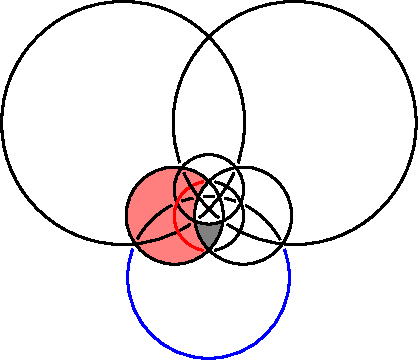
\includegraphics[scale=1]{probleme4}}
	\caption{A big problem in the proof...}
	\label{fig:problemVanish}
\end{figure}
We actually found similar problems in type~$B_3$...
\end{proof}

The following functions will play a fundamental role.

\begin{definition}
\label{def:forcingDominant}
A function~$f : \allShards \to \R_{>0}$ is \defn{forcing dominant} if for any two adjacent regions~$\region, \region' \in \posetRegions$ with~${\rays[\region] \ssm \{\ray\} = \rays[\region'] \ssm \{\ray'\}}$ and separated by the whard~$\sepShard$,
%\[
%\sum_{\ray[s] \in \rays[\region \,\cup\, \region']} \coefficient(\region, \region', \ray[s]) \sum_{\shard \in \allShards} f(\shard) \, \contribution(\shard, \ray[s]) > 0.
%\]
%%\[
%%\sum_{\ray[s] \in \rays[\region \,\cup\, \region']} \coefficient(\region, \region', \ray[s]) \sum_{\shard \in \shards} f(\shard) \, \contribution(\shard, \ray[s]) > 0.
%%\]
%%for any subset~$\shards \subseteq \allShards$ containing~$\sepShard$.
\[
f(\sepShard) > \frac{1}{\coefficient(\region, \region', \ray[r]) \, \contribution(\sepShard, \ray[r]) + \coefficient(\region, \region', \ray[r]') \, \contribution(\sepShard, \ray[r]')} \sum_{\ray[s] \in \rays[\region \,\cup\, \region']} |\coefficient(\region, \region', \ray[s])| \sum_{\shard \prec \sepShard} f(\shard) \, \contribution(\shard, \ray[s]).
\]
\end{definition}

Note that in Definition~\ref{def:forcingDominant}, we have
\[
\coefficient(\region, \region', \ray[r]) \, \contribution(\sepShard, \ray[r]) + \coefficient(\region, \region', \ray[r]') \, \contribution(\sepShard, \ray[r]') > 0
\]
since~$\contribution(\sepShard, \ray[r]) > 0$ and~$\contribution(\sepShard, \ray[r]') > 0$ by Lemma~\ref{lem:contribution}\,(i), and~$\coefficient(\region, \region', \ray[r]) > 0$ and~$\coefficient(\region, \region', \ray[r]') > 0$ by the choice of~$\coefficient$.

\begin{lemma}
Forcing dominant functions exist when the poset of regions~$\posetRegions$ is congruence uniform.
\end{lemma}

\begin{proof}
Since the poset of regions~$\posetRegions$ is congruence uniform, Theorem~\ref{thm:forcingAcyclic} ensures that the forcing relation~$\succ$ on~$\allShards$ is acyclic.
We can therefore fix the values of~$f$ in the order given by the forcing relation~$\succ$. For a given shard~$\shard_\bullet$, we choose~$f(\shard_\bullet)$ large enough so that for any pairs~$\region, \region'$ of adjacent regions of~$\arrangement$ separated by~$\shard_\bullet$, we have
\[
f(\shard_\bullet) > \frac{1}{\coefficient(\region, \region', \ray[r]) \, \contribution(\shard_\bullet, \ray[r]) + \coefficient(\region, \region', \ray[r]') \, \contribution(\shard_\bullet, \ray[r]')} \sum_{\ray[s] \in \rays[\region \,\cup\, \region']} |\coefficient(\region, \region', \ray[s])| \sum_{\shard \prec \shard_\bullet} f(\shard) \, \contribution(\shard, \ray[s])
\]
This is possible since~${\coefficient(\region, \region', \ray[r]) \, \contribution(\shard_\bullet, \ray[r]) + \coefficient(\region, \region', \ray[r]') \, \contribution(\shard_\bullet, \ray[r]')}$ is positive, and there are only finitely many pairs~$\region, \region'$ of adjacent regions of~$\arrangement$ separated by~$\shard_\bullet$.
\end{proof}

%%The term forcing dominant might not be evident in Definition~\ref{def:forcingDominant}
%
%\begin{lemma}
%Forcing dominant functions exist when the poset of regions~$\posetRegions$ is congruence uniform.
%\end{lemma}
%
%\begin{proof}
%Since the poset of regions~$\posetRegions$ is congruence uniform, Theorem~\ref{thm:forcingAcyclic} ensures that the forcing relation~$\succ$ on~$\allShards$ is acyclic.
%We fix the values of~$f$ in the order given by the forcing relation~$\succ$ and choose~$f(\shard)$ large enough so that for any pairs~$\region, \region'$ of adjacent regions of~$\arrangement$ separated by~$\shard$, we have
%\[
%f(\shard) > \frac{-1}{\coefficient(\region, \region', \ray[r]) \contribution(\shard, \ray[r]) + \coefficient(\region, \region', \ray[r]') \contribution(\shard, \ray[r]')} \sum_{\ray[s] \in \rays[\region \,\cup\, \region']} |\coefficient(\region, \region', \ray[s])| \sum_{\shard' \prec \shard} f(\shard') \, \contribution(\shard', \ray[s])
%\]
%where~$\rays[\region] \ssm \{\ray[r]\} = \rays[\region'] \ssm \{\ray[r]'\}$.
%Note that 
%\[
%\coefficient(\region, \region', \ray[r]) \contribution(\shard, \ray[r]) + \coefficient(\region, \region', \ray[r]') \contribution(\shard, \ray[r]') > 0
%\]
%since~$\contribution(\shard, \ray[r]) > 0$ and~$\contribution(\shard, \ray[r]') > 0$ by Lemma~\ref{lem:contribution}\,(i), and~$\coefficient(\region, \region', \ray[r]) > 0$ and~$\coefficient(\region, \region', \ray[r]') > 0$ by the choice of~$\coefficient$. Moreover, since~$\shard = \sepShard$, we have by Lemma~\ref{lem:contribution}\,(i)
%\[
%\sum_{\ray[s] \in \rays[\region \,\cup\, \region']} \coefficient(\region, \region', \ray[s]) \, \contribution(\shard, \ray[s]) = \coefficient(\region, \region', \ray[r]) \contribution(\shard, \ray[r]) + \coefficient(\region, \region', \ray[r]') \contribution(\shard, \ray[r]').
%\]
%By Lemma~\ref{lem:contribution}\,(ii), it follows that
%\begin{align*}
%\sum_{\ray[s] \in \rays[\region \,\cup\, \region']} \coefficient(\region, \region', \ray[s]) \sum_{\shard' \in \allShards} f(\shard') \, \contribution(\shard', \ray[s])
%& =
%\big[ \coefficient(\region, \region', \ray[r]) \contribution(\shard, \ray[r]) + \coefficient(\region, \region', \ray[r]') \contribution(\shard, \ray[r]') \big] \, f(\shard) \\
%& \;\; + \sum_{\ray[s] \in \rays[\region \,\cup\, \region']} \coefficient(\region, \region', \ray[s]) \sum_{\shard' \succ \shard} f(\shard') \, \contribution(\shard', \ray[s]) \\
%& > 0
%\end{align*}
%by the choice of~$f(\shard)$.
%In other words, $f$ is forcing dominant.
%\end{proof}

From now on, we fix a forcing dominant function~$f : \allShards \to \R_{>0}$.
We now consider a lattice congruence~$\equiv$ of the poset of regions~$\posetRegions$.
We define the \defn{height function}~$\height : \rays[\arrangement] \to \R_{>0}$~by
\[
\height(\ray[s]) \; \eqdef \sum_{\shard \in \shardsEquiv} f(\shard) \, \gamma(\shard, \ray[s]).
\]
This height function fulfills the following property.

\begin{lemma}
\label{lem:inequality}
For any two adjacent regions~$\region, \region' \in \posetRegions$, we have
\[
\sum_{\ray[s] \in \rays[\region \,\cup\, \region']} \coefficient(\region, \region', \ray[s]) \, \height(\ray[s]) \ge 0.
\]
with equality if and only if $\region$ and~$\region'$ belong to the same cone of~$\fanEquiv$. %$\sepShard \notin \shardsEquiv$.
\end{lemma}

\begin{proof}
%We have
%\[
%\sum_{\ray[s] \in \rays[\region \,\cup\, \region']} \coefficient(\region, \region', \ray[s]) \, \height(\ray[s]) = \sum_{\shard \in \shardsEquiv} f(\shard) \sum_{\ray[s] \in \rays[\region \,\cup\, \region']} \coefficient(\region, \region', \ray[s]) \, \gamma(\shard, \ray[s]).
%\]
Reorganizing the sums and applying Lemma~\ref{lem:contribution}\,(ii), we obtain
\[
\sum_{\ray[s] \in \rays[\region \,\cup\, \region']} \coefficient(\region, \region', \ray[s]) \, \height(\ray[s]) = \sum_{\substack{\shard \in \shardsEquiv \\ \shard \preccurlyeq \sepShard}} f(\shard) \sum_{\ray[s] \in \rays[\region \,\cup\, \region']} \coefficient(\region, \region', \ray[s]) \, \gamma(\shard, \ray[s]).
\]
We now distinguish two cases.
\begin{itemize}
\item Assume first that $\region$ and~$\region'$ belong to the same cone of~$\fanEquiv$. Then $\set{\shard \in \shardsEquiv}{\shard \preccurlyeq \sepShard}$ is empty since~$\sepShard \notin \shardsEquiv$ and~$\shardsEquiv$ is an upper ideal of the forcing order. Therefore, the sum is empty and we obtain
\[
\qquad\qquad
\sum_{\ray[s] \in \rays[\region \,\cup\, \region']} \coefficient(\region, \region', \ray[s]) \, \height(\ray[s]) = 0.
\]
\item Assume now that $\region$ and~$\region'$ belong to distinct cones of~$\fanEquiv$. Then~$\sepShard \notin \shardsEquiv$ and we have
\begin{align*}
\qquad\qquad
\sum_{\ray[s] \in \rays[\region \,\cup\, \region']} \coefficient(\region, \region', \ray[s]) \, \height(\ray[s]) & > \big( \coefficient(\region, \region', \ray[r]) \contribution(\sepShard, \ray[r]) + \coefficient(\region, \region', \ray[r]') \contribution(\sepShard, \ray[r]') \big) \, f(\sepShard) \\[-.4cm]
& \qquad - \sum_{\ray[s] \in \rays[\region \,\cup\, \region']} |\coefficient(\region, \region', \ray[s])| \sum_{\shard \prec \sepShard} f(\shard) \, \contribution(\shard, \ray[s]) \\
& > 0
\end{align*}
since~$f$ is forcing dominant.
\qedhere
\end{itemize}
\end{proof}

\begin{corollary}
Consider a simplicial hyperplane arrangement~$\arrangement$ and a base region~$\region[B]$ such that the poset of regions~$\posetRegions$ is congruence uniform.
Then for any lattice congruence of the poset of region~$\posetRegions$ and any forcing dominant function~$f : \allShards \to \R_{>0}$, the quotient fan~$\fanEquiv$ is the normal fan of the polytope
\[
\quotientope \eqdef \bigset{\b{x} \in \R^n}{\dotprod{\ray}{\b{x}} \le \height(\ray) \text{ for all } \ray \in \rays}.
\]
In particular, the graph of~$\quotientope$ oriented in a linear direction from~$\region[B]$ to~$-\region[B]$ is the Hasse diagram of the quotient~$\posetRegions/{\equiv}$.
\end{corollary}

\begin{proof}
We just combine the polytopality criterion of Proposition~\ref{prop:polytopalSubfanFan} with the inequality of Lemma~\ref{lem:inequality} to obtain the polytopality of the quotient fan~$\fanEquiv$.
The end of the statement then follows from~Theorem~\ref{thm:fanQuotient}.
\end{proof}

We call \defn{quotientope} the resulting polytope~$\quotientope$.
See Figures~\ref{fig:permAssoCube} and~\ref{fig:relevantQuotientopes} for illustrations.
\vincent{Add illustrations}
Note that not all quotientopes are simple since not all quotient fans are simplicial.

\begin{remark}
Is is tempting to extend Theorem~\ref{thm:quotientopes} to any (non-necessarily simplicial) arrangement whose poset of regions is a lattice.
However, our method cannot be adapted directly as our proof strongly relies on Proposition~\ref{prop:polytopalSubfanFan} where~$\Fan$ needs to be simplicial.
The first situation to consider is certainly when the arrangement is tight with respect to the base region.
\end{remark}


\begin{figure}[h]
	\capstart
	\centerline{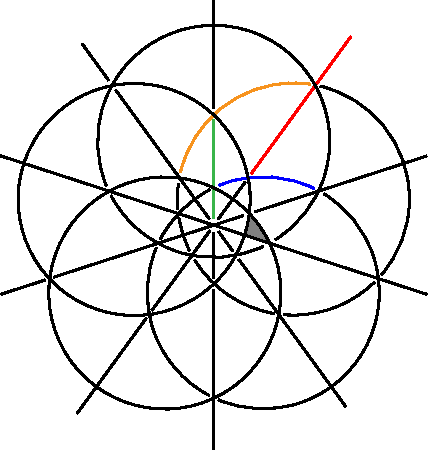
\includegraphics[scale=1]{probleme2} \quad 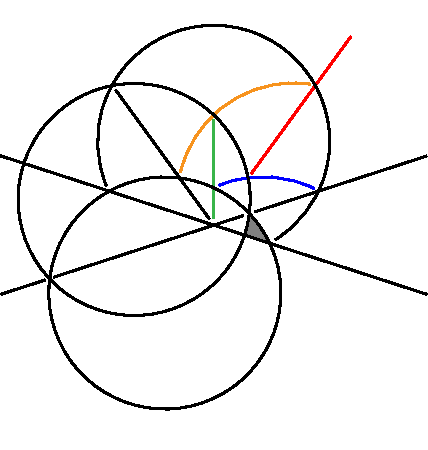
\includegraphics[scale=1]{probleme3}}
	\caption{(Left) A simplicial hyperplane arrangement~$\arrangement$ with a base region~$\region[B]$ such that~$\posetRegions$ is not congruence uniform. The four colored shards form a cycle for the forcing relation~$\succ$. (Right) Is this lattice quotient fan polytopal?}
	\label{fig:problems}
\end{figure}

\vincent{Understand this example}


%%%%%%%%%%%%%%%%%%%%%%%%%%%%%%%%%%%%%%

%\addtocontents{toc}{\vspace{.3cm}}
%\section*{Acknowledgements}

%%%%%%%%%%%%%%%%%%%%%%%%%%%%%%%%%%%%%%

\bibliographystyle{alpha}
\bibliography{quotientopes}
\label{sec:biblio}

\end{document}
